%%%%%%%%%%%%%%%%%%%%%%%%%%%%%%%%%%%%%%%%%%%%%%%%%%%%%%%%%%%%%%%%%%%%%%%%%%%%%%
%
% MASTER FILE START
%
%%%%%%%%%%%%%%%%%%%%%%%%%%%%%%%%%%%%%%%%%%%%%%%%%%%%%%%%%%%%%%%%%%%%%%%%%%%%%%

\RequirePackage{ifpdf}
\ifpdf
  \documentclass[ignoreframetext,envcountsect]{beamer}
\else
  \documentclass[ignoreframetext,dvips,trans,envcountsect]{beamer}
\fi

%%%%%%%%%%%%%%%%%%%%%%%%%%%%%%%%%%%%%%%%%%%%%%%%%%%%%%%%%%%%%%%%%%%%%%%%%%%%%%
%
% PACKAGES
%
%%%%%%%%%%%%%%%%%%%%%%%%%%%%%%%%%%%%%%%%%%%%%%%%%%%%%%%%%%%%%%%%%%%%%%%%%%%%%%

\usepackage[]{fontenc}         % select new font encodings
\usepackage[utf8]{inputenc}  % select input encoding
\usepackage{fancybox}          % nice boxes
\usepackage{ifpdf}             % using the ifpdf conditional
\usepackage{alltt}             % use tex-environments inside verbatim
\usepackage{epsfig}            % another way to include eps-figures
\usepackage{epic,eepic}        % extended picture environments 
\usepackage{graphicx,color}    % support for including graphics
\usepackage{latexsym}          % symbols
\usepackage{xspace}            % intelligent space after macros
\usepackage{url}               % url typeset correctly
\usepackage{epstopdf}          % on-the-fly conversion of eps to pdf when needed
\usepackage{lmodern}
\DeclareGraphicsRule{.pdftex}{pdf}{.pdftex}{}
\usepackage{bibentry}
\usepackage{amstext,amssymb,amsbsy}
\usepackage{amsmath}
\usepackage{pifont}

\usepackage{proof}
\usepackage[normalem]{ulem}

\usepackage{slidesec}

\mode<article>
{
\usepackage{fullpage}
}


\newcommand{\sa}[0]{\textrm{a}}
\newcommand{\se}[0]{\textrm{e}}
\newcommand{\si}[0]{\textrm{i}}
\newcommand{\so}[0]{\textrm{o}}
\renewcommand{\sa}[0]{\mbox{$\mathrm{a}$}}
\renewcommand{\se}[0]{\mbox{$\mathrm{e}$}}
\renewcommand{\si}[0]{\mbox{$\mathrm{i}$}}
\renewcommand{\so}[0]{\mbox{$\mathrm{o}$}}
\nobibliography*
\let\newblock\relax


%%%%%%%%%%%%%%%%%%%%%%%%%%%%%%%%%%%%%%%%%%%%%%%%%%%%%%%%%%%%%%%%%%%%%%%%%%%%%%
%
% CUSTOM BEAMER STYLE
%
%%%%%%%%%%%%%%%%%%%%%%%%%%%%%%%%%%%%%%%%%%%%%%%%%%%%%%%%%%%%%%%%%%%%%%%%%%%%%%

\useoutertheme{infolines}

\setbeamersize{text margin left=0.5cm}
\setbeamersize{text margin right=0.5cm}
\setbeamercovered{invisible}

%\definecolor{orange}{cmyk}{0,0.61,0.87,0}

\newcommand{\emptyhead}{\vskip-4pt
       \leavevmode
       \hbox{
       \begin{beamercolorbox}[wd=.96\paperwidth,leftskip=3ex]{title in head/foot}
       \color{bg}
       Empty Head
       \hfill
       \end{beamercolorbox}
       }
       \vskip0.75pt
}

\newcommand{\myhead}{\vskip-4pt
       \leavevmode
       \hbox{
       \begin{beamercolorbox}[wd=.48\paperwidth,leftskip=3ex]{title in head/foot}
       \insertpart
       \hfill
       \end{beamercolorbox}
       \hfill
       \begin{beamercolorbox}[wd=.48\paperwidth,rightskip=3ex]{title in head/foot}
       \hfill
       \insertframenumber/\inserttotalframenumber
       \end{beamercolorbox}
       }
       \vskip0pt
}

\newcommand{\emptyfoot}{
       \leavevmode
       \hbox{
       \begin{beamercolorbox}[wd=.96\paperwidth,leftskip=3ex]{title in head/foot}
       \color{bg}
       Empty Foot
       \hfill
       \end{beamercolorbox}
       }
       \vskip9.75pt
}

\newcommand{\myfoot}{
       \leavevmode
       \hbox{
       \begin{beamercolorbox}[wd=.58\paperwidth,leftskip=3ex]{title in head/foot}
       \insertshorttitle
       \hfill
       \end{beamercolorbox}
       \hfill
       \begin{beamercolorbox}[wd=.38\paperwidth,rightskip=3ex]{navigation symbols}
       \hfill
       \ifpdf
       %\insertslidenavigationsymbol
       %\insertframenavigationsymbol
       %\insertsubsectionnavigationsymbol
       %\insertsectionnavigationsymbol
       %\insertdocnavigationsymbol
       %\insertbackfindforwardnavigationsymbol
       \fi
       \end{beamercolorbox}
       }
       \vskip9pt
}

\newcommand{\myfootalt}{
       \leavevmode
       \hbox{
       \begin{beamercolorbox}[wd=.38\paperwidth,leftskip=3ex]{navigation symbols}
       \ifpdf
       %\insertslidenavigationsymbol
       %\insertframenavigationsymbol
       %\insertsubsectionnavigationsymbol
       %\insertsectionnavigationsymbol
       %\insertdocnavigationsymbol
       %\insertbackfindforwardnavigationsymbol
       \fi
       \hfill
       \end{beamercolorbox}
       \hfill
       \begin{beamercolorbox}[wd=.58\paperwidth,rightskip=3ex]{title in head/foot}
       \hfill
       \insertframenumber/\inserttotalframenumber       
       \end{beamercolorbox}
       }
       \vskip9pt
}

\setbeamertemplate{navigation symbols}{}
%\setbeamertemplate{headline}{\myhead}
%\setbeamertemplate{footline}{\myfoot}
\setbeamertemplate{footline}{\myfootalt}
%\setbeamertemplate{footline}[text line]{}
%\setbeamertemplate{headline}[text line]{}
\setbeamertemplate{headline}{\emptyhead}
%\setbeamertemplate{footline}{\emptyfoot}


\setbeamertemplate{frametitle}{
\begin{centering}
    \insertframetitle\par
\end{centering}
}

\setbeamertemplate{part page}{
\begin{centering}
\begin{beamercolorbox}[wd=\paperwidth]{title in head/foot}
\begin{center}\vspace{2ex}\inserttitle\\[1ex]\insertpart\end{center}
\end{beamercolorbox}
\end{centering}
\begin{centering}
\insertauthor\par
\end{centering}
\begin{centering}
\vspace*{1.5ex}{\scriptsize \insertinstitute}\par
\end{centering}
\vspace*{2ex}\par
\begin{centering}
\insertdate
\end{centering}
}

\AtBeginPart{
\frame[plain]{\partpage}
\addtocounter{framenumber}{-1}
}

\mode<presentation>
{
\newtheorem{mybox}[]{}
}

\mode<article>
{
\newcommand{\mybox}{}
}


\newcommand{\blue}[1]{\textcolor{blue}{#1}}
%\newcommand{\blue}[1]{\textcolor{red!30!green!30!blue!90}{#1}}

\newcommand{\red}[1]{\textcolor{red}{#1}}
\ifpdf
  \newcommand{\yellow}[1]{\textcolor{orange}{#1}}
\else
  \newcommand{\yellow}[1]{\blue{#1}}
\fi
\newcommand{\green}[1]{\textcolor{green}{#1}}
\newcommand{\white}[1]{\textcolor{white}{#1}}
\newcommand{\black}[1]{\textcolor{black}{#1}}

\mode<handout|trans|article>
{
\renewcommand{\yellow}[1]{\blue{#1}}
}


\newcommand{\bluearrow}{\blue{\Pisymbol{pzd}{228}}}
\newcommand{\blueresarrow}{\large\blue{\Pisymbol{pzd}{229}}}
\newcommand{\greenarrow}{\green{\Pisymbol{pzd}{228}}}
\newcommand{\greenresarrow}{\large\green{\Pisymbol{pzd}{229}}}
\newcommand{\redarrow}{\red{\Pisymbol{pzd}{228}}}
\newcommand{\redresarrow}{\large\red{\Pisymbol{pzd}{229}}}
\newcommand{\yellowarrow}{\yellow{\Pisymbol{pzd}{228}}}
\newcommand{\yellowresarrow}{\large\yellow{\Pisymbol{pzd}{229}}}

\newcommand{\cemph}[1]{\yellow {\emph{#1}}}
%\newcommand{\myitem}{\item[\bluearrow]}
\newcommand{\myitem}{\item[\Pisymbol{pzd}{228}]}
\newcommand{\mi}{\myitem}
%\newcommand{\bitem}{\item[\blue {\textbf{--}}]}
\newcommand{\bitem}{\item[{\textbf{--}}]}
%\newcommand{\resitem}{\item[\blueresarrow]}
\newcommand{\resitem}{\item[\large{\Pisymbol{pzd}{229}}]}
\newcommand{\h}{\yellow {$\Longrightarrow$}}

\newcommand{\itarrow}{\yellow{\Pisymbol{pzd}{229}}}
\newcommand{\ithook}{\yellow{\Pisymbol{pzd}{52}}}
\newcommand{\itcross}{\yellow{\Pisymbol{pzd}{56}}}
\newcommand{\ithand}{\yellow{\Pisymbol{pzd}{43}}}


\newcommand{\gdw}[0]{~$\Longleftrightarrow$~}
\newcommand{\commadots}[0]{,\ldots ,}
\newcommand{\magenta}[1]{\textcolor{magenta}{#1}}
%\newcommand{\blue}[1]{\textcolor{blue}{#1}}
\renewcommand{\blue}[1]{\textcolor{red!30!green!30!blue!100}{#1}}
\renewcommand{\magenta}[1]{\textcolor{red}{#1}}
\newcommand{\Th}[1]{\mathit{Th}(#1)}
\newcommand{\hence}{\;\dot{.\;.}\;}
\newcommand{\quantifier}{{\sf Q}}
\newcommand{\dt}{T=\langle W,D\rangle}
\newcommand{\reduct}[2]{#1^{#2}}
\newcommand{\Cn}[1]{\Th{#1}}


\setbeamertemplate{itemize item}{\Pisymbol{pzd}{228}}
\setbeamertemplate{itemize subitem}{{$\bullet$}}
\setbeamertemplate{itemize subsubitem}{\textbf{--}}

%
% Use equal font size at all levels (of itemization and enumeration)
%
\setbeamerfont{itemize/enumerate subbody}{size=\normalsize}
\setbeamerfont{itemize/enumerate subsubbody}{size=\normalsize}
\setbeamerfont{itemize subitem}{size=\normalsize}
\setbeamerfont{itemize subsubitem}{size=\normalsize}
\setbeamerfont{enumerate subitem}{size=\normalsize}
\setbeamerfont{enumerate subsubitem}{size=\normalsize}


\mode<article>
{
\renewcommand{\labelitemi}{\blue{\Pisymbol{pzd}{228}}}
\renewcommand{\labelitemii}{\blue{$\bullet$}}
\renewcommand{\labelitemiii}{\blue{\textbf{--}}}
\renewcommand{\myitem}{\item[\bluearrow]}
\renewcommand{\bitem}{\item[\blue {\textbf{--}}]}
\renewcommand{\resitem}{\item[\blueresarrow]}

%%%%%%%%%%%%%%%%%%%%%%%%%%%%%%%%%%%%%%%%%%%%%%%%%%%%%%%%%%%%%%%%

}

\mode<handout|trans>
{
\beamertemplatenavigationsymbolsempty
}

\ifpdf
\else
\mode<beamer>
{
  \beamertemplatenavigationsymbolsempty
}
\fi


%%%%%%%%%%%%%%%%%%%%%%%%%%%%%%%%%%%%%%%%%%%%%%%%%%%%%%%%%%%%%%%%%%%%%%%%%%%%%%
%
% MACROS
%
%%%%%%%%%%%%%%%%%%%%%%%%%%%%%%%%%%%%%%%%%%%%%%%%%%%%%%%%%%%%%%%%%%%%%%%%%%%%%%

\def\AND     { \,\wedge\,                 }
\def\OR      { \,\vee\,                   }
\def\XOR     { \,\stackrel{.}{\vee}\,     }
\def\IMPLIES { \,\supset\,                }
\def\IMPL    { \,\supset\,                }
\def\IF      { \,\leftarrow\,             }
\def\IFF     { \,\equiv\,         }
\def\IFFdef  { \,\stackrel{\rm def}{\longleftrightarrow}\, }

\newcommand{\iec}[0]{i.e.,\ }
\newcommand{\egc}[0]{e.g.,\ }
\newcommand{\ra}[0]{\rightarrow}
\newcommand{\Ra}[0]{$\Rightarrow$\ }
\newcommand{\bi}[0]{\begin{itemize}\itemsep=+.5ex}
\newcommand{\ei}[0]{\end{itemize}}
\newcommand{\bdescr}[0]{\begin{description}}
\newcommand{\edescr}[0]{\end{description}}
\newcommand{\be}[0]{\begin{enumerate}\itemsep=+.5ex}
\newcommand{\ee}[0]{\end{enumerate}}

\newcommand\nop[1]{}
\newif\ifmakebbl
\newcommand{\sld}{\mode<presentation>}
\newcommand{\lns}{\mode<article>}



%%%%%%%%%%%%%% SPACING COMMANDS 

\newcommand{\nbls}{\vspace*{-1\baselineskip}}
\newcommand{\hnbls}{\vspace*{-.5\baselineskip}}
\newcommand{\tnbls}{\vspace*{-.33\baselineskip}}
\newcommand{\qnbls}{\vspace*{-.25\baselineskip}}

\newcommand{\bls}{\vspace*{1\baselineskip}}
\newcommand{\hbls}{\vspace*{.5\baselineskip}}
\newcommand{\tbls}{\vspace*{.33\baselineskip}}
\newcommand{\qbls}{\vspace*{.25\baselineskip}}

\newcommand{\bs}{\bigskip}
\newcommand{\ms}{\medskip}
% \newcommand{\b}{\bigskip}
\newcommand{\m}{\medskip}
\newcommand{\s}{\smallskip}
\newcommand{\sm}{\smallskip}

%\input{macro.tex}

%%%%%%%%%%%%%%%%%%%%%%%%%%%%%%%%%%%%%%%%%%%%%%%%%%%%%%%%%%%%%%%%%%%%%%%%%%%%%%
%
% DOCUMENT PROPERTIES
%
%%%%%%%%%%%%%%%%%%%%%%%%%%%%%%%%%%%%%%%%%%%%%%%%%%%%%%%%%%%%%%%%%%%%%%%%%%%%%%

\title{Exercise 1}
\author[S. Mortezapoor,N. Rekabsaz,D. Rossegger]{Soroosh Mortezapoor, Navid Rekabsaz, Dino Rossegger}
\institute{VU Machine Learning WS 13/14}
\date[19.12.2013]{December, $19^{th}$, 2013}
\subject{Exercise 1}

%%%%%%%%%%%%%%%%%%%%%%%%%%%%%%%%%%%%%%%%%%%%%%%%%%%%%%%%%%%%%%%%%%%%%%%%%%%%%%
%
% DOCUMENT START
%
%%%%%%%%%%%%%%%%%%%%%%%%%%%%%%%%%%%%%%%%%%%%%%%%%%%%%%%%%%%%%%%%%%%%%%%%%%%%%%

\begin{document}

\frame[plain]{\titlepage}
\lns{\maketitle}

\addtocounter{framenumber}{-1}
 
%%%%%%%%%%%%%%%%%%%%%%%%%%%%%%%%%%%%%%%%%%%%%%%%%%%%%%%%%%%%%
%Themen
\begin{frame}{Datasets}
\bs
\bi
\mi Auto MPG\\
$398\times8$, missing values
\mi Year Prediction MSD\\
$515,345\times90$, no missing values
\mi Electric Power Consumption\\
$2,075,259\times9$, missing values
\ei

\end{frame}

\begin{frame}{Algorithms}
\bs
\bi
\mi Linear Ridge Regression
\mi $k$-nearest neighbors
\mi Support Vector Machines
\mi Stochastic Gradient Descent
\ms
\mi Polynomial Ridge Regression
\mi Neural Networks
\ei
\end{frame}

\begin{frame}{Framework}
\bs
\bi
\mi Python
\mi \textit{scikit-learn}\\
\url{http://scikit-learn.org}
\mi \textit{pybrain} for Neural Networks\\
\url{http://pybrain.org}
\mi \textit{datetime} for runtime measuring
\ei
\end{frame}

\section{Contraceptive Method Choice}
\label{db:sec:ds1}
\subsection{Description}
Contraceptive Method Choice ~\cite{ds1:uci} contains the results of a survey. The samples are married women who were either not pregnant or do not know if they were at the time of interview. The problem is to predict the current contraceptive method choice of a woman based on her demographic and socio-economic characteristics. The dataset has $9$ attributes and $1473$ samples. The dataset has no missing value. As it's mentioned, it has three classes: $1$ No-Use, $2$ Long-term method and $3$ Short-term method.

Different type of attributes such as binary, numerical and categorical as well as shortage of data make the dataset distinct and interesting for Machine Learning experiences.

\subsection{Preprocessing}
The dataset is split into three parts: $i$ Training dataset ($60\%$), $ii$ Validation dataset ($20\%$) and $iii$ Test dataset ($20\%$). As it's mentioned before, shuffling algorithms of Scikit-Learn is used for splitting the dataset.

In order to scale the data, we choose Zero Mean, Min Max and 1-N vector for encoding categorical data. In order to have a better overview of result of preprocessing, we use Principal Component Analysis (PCA). By using PCA algorithm provided by Scikit-Learn, we reduce dimension of data to two and draw plots by applying different techniques. 

As it is depicted in Figure \ref{ds1:fig:dimred}, the second plot seems too dense and unclear (as applying Zero-Mean on binary features may not be a good approach). By comparing the first and third plots, we can say that they seem very similar. Therefore, we use the first and the forth preprocessing method for the rest of the current section. By convention we call the first method (Numerical : Zero-Mean, Categorical : 1-N, Binary : None) $PreProc1$ and the second (Numerical : Min-Max, Categorical : 1-N, Binary : None) $PreProc2$.


\subsection{Logistic Regression}
We applied different values of the parameter $C$ (Inverse of regularization strength) and tried the algorithm in both polynomial and linear ways. Whole the process was also done using two preprocessing methods mentioned before.

The F1-score of the result is shown in Table\ref{ds1:table:logisticregression}. As it's shown in Table\ref{ds1:table:logisticregression}, changing the parameter $C$ doesn't cause any significant difference in results while $0.1$ seems to be slightly better. Also while $PreProc1$ seems better in result in some records, $PreProc2$ seems to be more stable and indifference against changing the highest exponent.


We applied the best result ($C=0.1$, $Highest exponent=10$) on test dataset and the result is shown in Table\ref{ds1:table:logisticregression-test}. The result is slightly worse than the best result of Validation dataset.


\subsection{Decision Tree}
We applied two criteria for decision tree: $gini$ and $entropy$. As before, we repeated it for two preprocessing methods mentioned before.

The F1-score of the result is shown in Table\ref{ds1:table:decisiontree}. $Gini$ seems to be a better criterion measure for the algorithm. Also in this case, $PreProc1$ seems better than $PreProc2$.

We applied again the best result ($Criterion=Gini$) on test dataset and the result is shown in Table\ref{ds1:table:decisiontree-test}. The result is again slightly worse than the best result of Validation dataset.

\subsection{$k$-nearest neighbor}
Since the data is so blended, we run the algorithm many times with different values of Number of Neighbors parameter. As before, the process is repeated two times for preprocessing methods.

The F1-score of the result is shown in Table\ref{ds1:table:knn}. Running the algorithm with $30$ neighbors as parameter seems to be the best result. Also in this case, $PreProc1$ seems better than $PreProc2$.

We applied again the best result ($Number of Neighbors=30$) on test dataset and the result is shown in Table\ref{ds1:table:knn-test}. The result is again slightly worse than the best result of Validation dataset.

\subsection{Support Vector Machine}
Kernel and value $C$ (Inverse of regularization strength) are two factors considered in running SVM algorithm. Different kernels like RBF (Radial Basis Function), Linear, Polynomial and Sigmoid are applied on the dataset.

Since the result of Sigmoid are significantly bad, in Table\ref{ds1:table:svm} we only show the results of RBF, Linear and Polynomial. Again $PreProc1$ seems better in result rather than $PreProc2$. As it's expected, RBF have the best results among other kernels.

We applied the best result ($C=1$, $Kernel=RBF$) on test dataset and the result is shown in Table\ref{ds1:table:svm-test}. The result is slightly worse than the best result of Validation dataset.

\subsection{Neural Networks}
Number of hidden layers as well as number of nodes in each hidden layer are two important factors in result of neural network algorithm. 

Usually the number of nodes in hidden layer should be at least twice as number of nodes in input layer (number of attributes). The results are shown in Table\ref{ds1:table:nn}. Again $PreProc1$ seems better in result rather than $PreProc2$. As it's expected, RBF have the best results among other kernels.

We applied the best result ($Number of Layers=1$, $Number of Nodes=120$) on test dataset. The result is shown in Table\ref{ds1:table:nn-test}. The result is as good as the best result of Validation dataset.

\subsection{Comparison}
Table\ref{ds1:table:comparison} compares the between best run of each algorithm on Test dataset based on the value of precision, recall, F1-score, learning time and prediction time.

Since SVM tends to have a better results among the other algorithm, its confusion matrix is depicted in Table \ref{ds1:table:confusionmatrix}
Based on achieved results, following points can be infered:
\begin{itemize}
\item Using Standard Deviation instead of MinMax leads to better results in all cases.
\item SVM has the best result and the result is rather consistent in different runs.
\item Surprisingly, KNN has a really good results such that it's completely comparable with SVM. Since it's a lazy learner algorithm, in the case of need it can be replaced with SVM.
\item Neural Network has a very bad result. Usually precision is better than recall and smaller collections are worse in results.
\item Analyzing confusion matrix and the results of runs show us that class $1$ and $3$ are mistaken more often. As it is mentioned before class $1$ and $3$ stand for No-use and Short-term.
\item While training and prediction time are usually less than one minute and not time consuming, NN algorithm tends to have about three times longer training time than the others.
\item Decision Tree is the fastest algorithm among the others
\item While KNN is expected to have a more prediction time than training, the same situation can be seen for Decision Tree. The reason is probably because of short amount of data and time which makes the situation not appropriate for judgment.
\end{itemize}

\begin{figure}[p]
\begin{center}
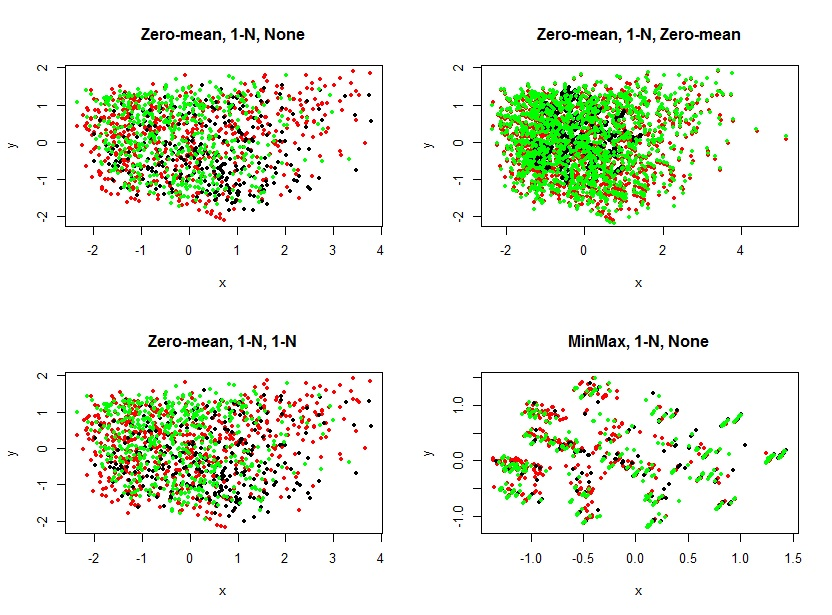
\includegraphics[scale=\figurescaling]{figures/db1/dim_reduction.jpg}
\caption{Dimensional Reduction applied on different preprocessing techniques (Numerical, Categorical, Binary)
\label{ds1:fig:dimred}}
\end{center}
\end{figure}


\begin{table}[p]
\begin{center}
\begin{tabular}{|c|c|c|c|c|}
\hline \multicolumn{2}{ |c| }{C} & 0.1 & 2 & 5 \\

\hline \multicolumn{1}{ |c| }{\multirow{6}{*}{Highest exponent} } & 1 & \minibox{0.50\\ 0.51} & \minibox{0.49 \\ 0.50} & \minibox{0.49 \\ 0.50} \\

\cline{2-5} & 5 & \minibox{0.55 \\ 0.53} & \minibox{0.55 \\ 0.52} & \minibox{0.56 \\ 0.53} \\

\cline{2-5} & 10 & \minibox{\textbf{0.56} \\ 0.50} & \minibox{0.54 \\ 0.51} & \minibox{0.54 \\ 0.52} \\

\cline{2-5} & 21 & \minibox{0.39 \\ 0.52} & \minibox{0.39 \\ 0.52} & \minibox{0.39 \\ 0.52} \\

\cline{2-5} & 33 & \minibox{0.34 \\ 0.52} & \minibox{0.34 \\ 0.52} & \minibox{0.34 \\ 0.53} \\

\cline{2-5} & 44 & \minibox{0.24 \\ 0.52} & \minibox{0.24 \\ 0.52} & \minibox{0.24 \\ 0.53} \\

\hline
\end{tabular}

\caption{Contraceptive Method Choice - Logistic Regressions F1-score ($PreProc1$, $PreProc2$)}
\label{ds1:table:logisticregression}
\end{center}
\end{table}


\begin{table}[p]
\begin{center}
\begin{tabular}{|c|c|c|c|c|}
\hline Class & Precision & Recall & F1-score & Support \\

\hline 0 & 0.59 & 0.62 & 0.60 & 126\\
\hline 1 & 0.54 & 0.22 & 0.32 & 67\\
\hline 2 & 0.46 & 0.61 & 0.53 & 102\\
\hline avg / total & 0.53 & 0.53 & 0.51 & 295\\
\hline
\end{tabular}

\caption{Contraceptive Method Choice - Logistic Regressions on Test dataset}
\label{ds1:table:logisticregression-test}
\end{center}
\end{table}

\begin{table}[p]
\begin{center}
\begin{tabular}{|c|c|}
\hline Criterion & F-Score \\

\hline Gini & \minibox{\textbf{0.48}\\ 0.47} \\

\hline Entropy & \minibox{0.46\\ 0.43} \\

\hline
\end{tabular}

\caption{Contraceptive Method Choice - Decision Tree F1-score ($PreProc1$, $PreProc2$)}
\label{ds1:table:decisiontree}
\end{center}
\end{table}


\begin{table}[p]
\begin{center}
\begin{tabular}{|c|c|c|c|c|}
\hline Class & Precision & Recall & F1-score & Support \\

\hline 0 & 0.55 & 0.57 & 0.56 & 126\\
\hline 1 & 0.33 & 0.34 & 0.34 & 67\\
\hline 2 & 0.42 & 0.39 & 0.41 & 102\\
\hline avg / total & 0.46 & 0.46 & 0.46 & 295\\
\hline
\end{tabular}

\caption{Contraceptive Method Choice - Decision Tree on Test dataset}
\label{ds1:table:decisiontree-test}
\end{center}
\end{table}


\begin{table}[p]
\begin{center}
\begin{tabular}{|c|c|}
\hline Number of Neighbors & F-Score \\

\hline 1 & \minibox{0.42\\ 0.45} \\
\hline 5 & \minibox{0.47\\ 0.46} \\
\hline 10 & \minibox{0.51\\ 0.43} \\
\hline 20 & \minibox{0.51\\ 0.45} \\
\hline 30 & \minibox{\textbf{0.56}\\ 0.47} \\
\hline 40 & \minibox{0.54\\ 0.49} \\
\hline 50 & \minibox{0.54\\ 0.47} \\

\hline
\end{tabular}

\caption{Contraceptive Method Choice - K Nearest Neighbors  F1-score ($PreProc1$, $PreProc2$)}
\label{ds1:table:knn}
\end{center}
\end{table}


\begin{table}[p]
\begin{center}
\begin{tabular}{|c|c|c|c|c|}
\hline Class & Precision & Recall & F1-score & Support \\

\hline 0 & 0.61 & 0.60 & 0.60 & 126\\
\hline 1 & 0.48 & 0.43 & 0.45 & 67\\
\hline 2 & 0.49 & 0.54 & 0.51 & 102\\
\hline avg / total & 0.54 & 0.54 & 0.54 & 295\\
\hline
\end{tabular}

\caption{Contraceptive Method Choice - K Nearest Neighbors on Test dataset}
\label{ds1:table:knn-test}
\end{center}
\end{table}


\begin{table}[p]
\begin{center}
\begin{tabular}{|c|c|c|c|c|c|c|}
\hline \multicolumn{2}{ |c| }{C} & 1 & 5 & 10 & 20 & 50 \\

\hline \multicolumn{1}{ |c| }{\multirow{2}{*}{Kernel} } & Linear & \minibox{0.48\\ 0.49} & \minibox{0.49 \\ 0.50} & \minibox{0.49 \\ 0.49} & \minibox{0.49 \\ 0.48} & \minibox{0.49 \\ 0.49} \\

\cline{2-7} & RBF & \minibox{\textbf{0.57} \\ 0.47} & \minibox{0.56 \\ 0.52} & \minibox{0.55 \\ 0.53} & \minibox{0.53 \\ 0.51}  & \minibox{0.52 \\ 0.51} \\

\cline{2-7} & Polynomial & \minibox{0.27 \\ 0.26} & \minibox{0.51 \\ 0.35} & \minibox{0.53 \\ 0.45} & \minibox{0.54 \\ 0.47}  & \minibox{0.53 \\ 0.48} \\

\hline
\end{tabular}

\caption{Contraceptive Method Choice - SVM F1-score ($PreProc1$, $PreProc2$)}
\label{ds1:table:svm}
\end{center}
\end{table}


\begin{table}[p]
\begin{center}
\begin{tabular}{|c|c|c|c|c|}
\hline Class & Precision & Recall & F1-score & Support \\

\hline 0 & 0.60 & 0.65 & 0.63 & 126\\
\hline 1 & 0.54 & 0.33 & 0.41 & 67\\
\hline 2 & 0.50 & 0.58 & 0.54 & 102\\
\hline avg / total & 0.55 & 0.55 & 0.55 & 295\\
\hline
\end{tabular}

\caption{Contraceptive Method Choice - SVM on Test dataset}
\label{ds1:table:svm-test}
\end{center}
\end{table}



\begin{table}[p]
\begin{center}
\begin{tabular}{|c|c|c|c|c|c|c|}
\hline \multicolumn{2}{ |c| }{Number of Nodes} & 30 & 60 & 90 & 120 & 150 \\

\hline \multicolumn{1}{ |c| }{\multirow{2}{*}{Number of Hidden Layers} } & 1 & \minibox{0.34\\ 0.28} & \minibox{0.27 \\ 0.32} & \minibox{0.35 \\ 0.32} & \minibox{\textbf{0.37} \\ 0.34} & \minibox{0.26 \\ 0.35} \\

\cline{2-7} & 2 & \minibox{0.18 \\ 0.18} & \minibox{0.26 \\ 0.18} & \minibox{0.26 \\ 0.26} & \minibox{0.26 \\ 0.18}  & \minibox{0.26 \\ 0.08} \\

\hline
\end{tabular}

\caption{Contraceptive Method Choice - Neural Network F1-score ($PreProc1$, $PreProc2$)}
\label{ds1:table:nn}
\end{center}
\end{table}


\begin{table}[p]
\begin{center}
\begin{tabular}{|c|c|c|c|c|}
\hline Class & Precision & Recall & F1-score & Support \\

\hline 0 & 0.53 & 0.26 & 0.35 & 126\\
\hline 1 & 0.26 & 0.42 & 0.32 & 67\\
\hline 2 & 0.37 & 0.46 & 0.41 & 102\\
\hline avg / total & 0.42 & 0.37 & 0.37 & 295\\
\hline
\end{tabular}
\caption{Contraceptive Method Choice - Neural Network on Test dataset}
\label{ds1:table:nn-test}
\end{center}
\end{table}



\begin{table}[p]
\begin{center}
\begin{tabular}{|p{5cm}|c|c|c|p{2cm}|p{2cm}|}
\hline Algorithm & Precision & Recall & F1-score & Training Time & Prediction Time \\
\hline Logistic Regression, PreProc1, C=0.1, Exponent=10 & 0.53 & 0.53 & 0.51 & 01.528 & 00.323\\
\hline Decision Tree, PreProc1, Criterion=Gini & 0.46 & 0.46 & 0.46 & \textbf{00.019} & \textbf{00.049}\\
\hline K Nearest Neighbors, PreProc1, NN=30 & 0.54 & 0.54 & 0.54 & 00.029 & 00.662 \\
\hline SVM, PreProc1, Kernel=RBF, C=1 & \textbf{0.55} & \textbf{0.55} & \textbf{0.55} & 00.281 & 00.189\\
\hline Neural Network, PreProc1, NL=1, NN=120 & 0.42 & 0.37 & 0.37 & 03.202 & 00.251\\
\hline
\end{tabular}
\caption{Contraceptive Method Choice - Comparison}
\label{ds1:table:comparison}
\end{center}
\end{table}


\begin{table}[p]
\begin{center}
\begin{tabular}{|c|c|c|c|}
\hline \backslashbox{Class}{Predicted} & 1 & 2 & 3  \\
\hline 1 & \textbf{80} & 9 & 37\\
\hline 2 & 16 & \textbf{28} & 23\\
\hline 3 & 30 & 11 & \textbf{60}\\
\hline
\end{tabular}
\caption{Contraceptive Method Choice - Confusion Matrix}
\label{ds1:table:confusionmatrix}
\end{center}
\end{table}


\section{First Order Theorem Proving}
\label{db:sec:ds2}
\subsection{Description}
This dataset First Order Theorem Proving~\cite{ds2:uci}~\cite{ds2:paper} is made of $6112$ instances made of $51$ attributes each. This $51$ attributes are static and dynamic features of first order theorems which were tried to be solved with $5$ different heuristics. The last $5$ columns contain the runtime of the heuristics or $-100$ if the heuristic was not able to prove the theorem within $100$ seconds.\par
Our first idea was to assign a class $1-5$ to each instance indicating which heuristic was the fastest or $0$ if the theorem could not be proved by any heuristic within $100$ seconds. Running experiments with this configuration we observed that all our machine learning algorithms did not produce any good results. While the hit rate for instances which were unsolvable was quite good, it seemed impossible to predict which heuristic was the fastest in most cases. Therefore we could not achieve a precision higher than $60\%$.
Looking at the instances the cause of this became obvious. For most of the provable theorems the difference in runtime of the heuristic was very small, in some cases all five of them had the same runtime. While this would not matter in practice since it is irrelevant which heuristic is chosen if all perform the same for our experiments we found it to be a little underwhelming. Therefore we changed our configuration, assigning classes to the instances based on the runtime of the best heuristic. The classes can be seen in Table~\ref{ds2:table:classes}.
\par The runtimes of all the algorithms tested were around $1$ second each and did not differ noticeably therefore detailed reporting is generally omitted.
\begin{table}[h]
	\begin{center}
	\begin{tabular}{c|c|c|c|c|c|c} 

		Label & $0$ & $1$ & $2$ & $3$ & $4$ & $5$\\\hline
		Runtime (s) & $>100$ & $<1$ & $<10$ & $<25$ & $<50$ &$<100$\\\hline
		$\#$ of instances & $2554$ & $2794$ & $504$ & $106$ & $77$ & $83$\\\hline
		percentage & $0.42$ & $0.46$ & $0.08$ & $0.02$ & $0.01$ & $0.01$\\\hline

	\end{tabular}
\end{center}
	\caption{Class assignment \label{ds2:table:classes}}
\end{table}
\subsection{Preprocessing}
We applied min max scaling as well as mean removal and variance scaling. It turned out that mean removal and variance scaling was the best scaling method. Imputation of missing values was not needed for this dataset but two attributes were removed because of redundancy. A test and validation dataset was used to tune the algorithms, $60\%$ of the dataset were used for training, $20\%$ were used for testing and validation respectively. 
\subsection{Logistic Regression}
Logistic Regression was applied with different parameters for the Regularization Strength ranging from $0.1$ to $5$. However changes in the parameters only minimally affected the quality of the model. Since the results only differed slightly in recall ($~0.01\%$) only the result of the best configuration is shown in Table~\ref{ds2:table:lr}. Interestingly Logistic Regression was not able to correctly classify instances of classes $3$ to $5$. This was the case with most of the algorithms, an intuitive explanation is given in Section~\ref{ds2:sec:comparison}. The model achieved similar results on the validation dataset.

\begin{table}[p]
\begin{center}
\begin{tabular}{|c|c|c|c|c|}
\hline Class & Precision & Recall & F1-score & Support \\
\hline  $0$    &   $0.60$    & $ 0.65$  &   $ 0.62$  &     $639$ \\
\hline  $1$    &   $0.61$    &  $0.74$  &   $ 0.67$  &     $699$ \\
\hline  $2-5$  &   $0.00$    &  $0.00$  &    $0.00$  &     $*$ \\
\hline avg / total &      $0.53$  &    $0.61$  &    $0.57$  &   $1531$\\
\hline
\end{tabular}

\caption{Result of Logistic Regression with $C=2$}
\label{ds2:table:lr}
\end{center}
\end{table}


\subsection{Decision Tree}
Decision Tree was applied with two different classification criterias \textit{gini} and \textit{entropy}. Both of them achieved similar results (F1-score difference $~0.01\%$) but with different results in the classes. The F1-score for the different criterias can be seen in Table~\ref{ds2:table:dtf1}. Interestingly Decision Tree was one of the few algorithms to classify some instances of class $3-5$ correctly. Still the result for this $3$ classes is still quite bad. The algorithms had similar performance on the validation dataset.
\begin{table}[p]
	\begin{center}
		\begin{tabular}{|c|c|c|c|c|c|c|c|}
\hline Class & $0$ & $1$ & $2$ & $3$ &$4$  &$ 5$ & total \\
\hline gini & $0.75$ &$0.74$ &$0.34$ &$0.14$&$0.11$&$0.26$&$0.69$\\
\hline entropy & $0.74$&$0.74$&$0.33$&$0.14$&$0.14$&$0.26$&$0.68$\\
\hline
	\end{tabular}


	\end{center}
	\caption{F1-Scores of Decision Tree with different classification criteria\label{ds2:table:dtf1}}
\end{table}
\subsection{$k$-nearest neighbor}
$k$-nearest neighbors was tested with $k \in [1,50]$. The choice of $k$ affected the result with $k=1$ being the best choice. A comparison of the F1-scores can be seen in Table~\ref{ds2:table:knnf1}. Interestingly the F1-score gets better the higher $k$ is chosen for class $3$ while it becomes worse for all the other classes. Both precision and recall are considerably better in $k=50$ for this class compared to $k=1$
being $0.4$ and $0.3$ compared to $0.12$ and $0.10$. This might also be because of the characteristics of the test set since this happened to less extent on the validation set. Apart from this the algorithms had similar performance on the validation set.
\begin{table}[p]
	\begin{center}
		\begin{tabular}{|c|c|c|c|c|c|c|c|}
\hline Class & $0$ & $1$ & $2$ & $3$ &$4$  &$ 5$ & total \\
\hline $1$ & $0.76$ & $0.76$ & $0.26$ & $0.11$ & $0.11$ & $0.33$ & $0.69$ \\
\hline $5$ & $0.74$ & $0.74$ & $0.14$ & $0.07$ & $0.09$ & $0.00$ & $0.66$ \\
\hline $10$ & $0.73$ & $0.75$ &$0.18$ & $0.07$ & $0.00$ & $0.19$ & $0.66$ \\
\hline $20$ & $0.72$ & $0.74$ &$0.18$ & $0.21$ & $0.00$ &	$0.00$ & $0.65$ \\
\hline $30$ & $0.69$ & $0.72$ &$0.24$ & $0.27$ & $0.00$ & $0.00$ & $0.64$ \\
\hline $40$ & $0.68$ & $0.71$ &$0.26$ &	$0.27$ & $0.00$ & $0.00$ & $0.64$ \\
\hline $50$ & $0.69$ & $0.72$ &$0.25$ & $0.34$ & $0.00$ & $0.00$ & $0.64$ \\
\hline
	\end{tabular}
	\end{center}
	\caption{F1-Scores of $k$-nearest neighbor with different $k$\label{ds2:table:knnf1}}
\end{table}
\subsection{Support Vector Machines}
Experiments with three different kernels, $rbf,linear,poly$ and different parameters for the penalty were done. Linear and polynomial support vector machines did not terminate within reasonable time and therefore reports on their performance are omitted. One run of linear support vector machines with $0.1$ as penalty finished successfully and it could be observed that the results were very bad. The penalty varied between $0.1$ and $100$ and while the performance on some classes varied, the overall performance stayed the same. The F1-scores of the configurations can be seen in Table~\ref{ds2:table:svmf1}. It can be seen that support vector machines with penalty $10$ and $5$ performed slightly better with $10$ being better in classifying theorems of the second class. This observation is backed up by the experiments on the validation data set where the same can be observed.
\begin{table}[p]
	\begin{center}
		\begin{tabular}{|c|c|c|c|c|c|c|c|}
\hline Class & $0$ & $1$ & $2$ & $3$ &$4$  &$ 5$ & total \\
\hline $0.1$ & $0.62$ & $0.72$ & $0.17$ & $0$ & $0$ & $0$ & $0.60$ \\
\hline $1$ & $0.71$ & $0.75$ & $0.27$ & $0$ & $0$ & $0$ & $0.66$ \\
\hline $5$ & $0.74$ & $0.76$ &$0.28$ & $0.12$ & $0$ & $0$ & $0.68$ \\
\hline $10$ & $0.74$ & $0.75$ &$0.28$ & $0.12$ & $0.00$ &	$0.00$ & $0.68$ \\
\hline $20$ & $0.73$ & $0.75$ &$0.25$ & $0.12$ & $0.00$ & $0.00$ & $0.67$ \\
\hline $50$ & $0.74$ & $0.74$ &$0.27$ & $0.12$ & $0.10$ & $0.00$ & $0.67$ \\
\hline
	\end{tabular}
	\end{center}
	\caption{F1-Scores of Support Vector Machines with kernel $rbf$ and different penalty\label{ds2:table:svmf1}}
\end{table}

\subsection{Neural Networks}
Experiments were done with different number of hidden layers and different number of nodes. Interestingly neither of the parameters made any difference in the result. In general the result obtained was very bad, only predicting instances in class $0$ correctly. Even in this class the algorithm only achieved a precision of $0.42$ but at least the recall was very good, being $1.00$. Similar results were obtained using the test set. The different configurations used where $1,2,3,4$ hidden layers and $300,600,900,1200$ nodes. 
\subsection{Comparison}
Decision trees and $k$-nearest neighbor with $k=1$ gave the best result with a F$1$-score of $0-69$. Apart from getting the higher F$1$-score overall, they were also able to classify instances with labels $3-5$ correctly which most of the other algorithms could not. Most of the other algorithms despite \textit{neural networks} fell only	$1-4\%$ short.
Looking at the class distribution visualized in Table~\ref{ds2:table:classes} it becomes obvious why all of the algorithms had problems labeling instances of the classes $2-5$ correctly since the number of instances labelled this way is very small, having only $~5\%$ of the dataset. The confusion matrix for decision trees with \textit{entropy} as classification criteria can be seen in Table~\ref{ds2:confmatrix}. It is highly visible that for classes $2-5$ it was very hard to do a correct prediction because of the small amount of data available. Most incorrectly-assigned labels where labelled with class $0$ or $1$, classes which contain many data.
\par \textit{Neural networks} was by far the worst classification technique being immune to parameter change and giving bad results in the validation as well as in the test dataset.

\begin{table}[p]
	\begin{center}
		\begin{tabular}{|c|c|c|c|c|c|c|}
		\hline	\backslashbox{Class}{Predicted} & $0$ & $1$ & $2$ & $3$ & $4$ & $5$ \\
		\hline  0 & $351$ & $94$ & $14$ & $8$ & $9$ & $3$ \\
		\hline  1 & $100$ & $389$ & $23$ & $5$ & $5$ & $2$ \\
		\hline  2 & $34$  & $33$ & $19$ & $4$ & $4$ & $1$ \\
		\hline  3 & $6$   & $3$ & $1$ & $5$ & $5$ & $0$ \\
		\hline  4 & $1$   & $2$ & $6$ & $3$ & $3$ & $0$ \\
		\hline  5 & $8$   & $2$ & $2$ & $0$ & $1$ & $3$ \\
		\end{tabular}
	\end{center}
		\caption{Confusion Matrix for Decision Tree with \textit{entropy}\label{ds2:confmatrix}}
\end{table}
\label{ds2:sec:comparison}

\section{third dataset}
While we had the possibility to test a lot of algorithms on AutoMPG~\ref{db:sec:ds1}, it was very hard if not impossible to achieve good results. We think that this is because of the small size of the training and test data, the missing values further complicate the appliance of machine learning. Although we saw differences between the algorithms, we have to conclude that even the best of them did not give very good predictions.\par
For Year Prediction MSD~\ref{db:sec:ds2} and Electric Power Consumption~\ref{db:sec:ds3} different algorithm performed best. Although the number of samples was much higher in EPC the lack of attributes compared to YPMSD seemed to have a big impact on the performance of the algorithms. While $k$-nearest neighbors worked very well for EPC, not only was it surpassed in terms of quality by other algorithms in YPMSD also its runtime was considerably worse compared to the other algorithms. This seems rational since the number of samples does not have a big impact on runtime of $k$-nearest neighbors in the implementation used by \textit{scikit}.\par
Despite the differences between the two datasets all algorithms generated reasonably good models only differing slightly in quality. We could not use Support Vector Machines any of these two datasets because of its huge runtime which is dependent on the number of samples.\par

It was also very interesting to see that for Stochastic Gradient Descent different $\epsilon$ performed best for the different datasets. While small $\epsilon$ resulted in very bad models for YPMSD it was a good choice for EPC and also on AutoMPG Stochastic Gradient Descent worked better with small $\epsilon$. Another interesting observation was that the choice of $\alpha$ did not have impact on model quality and had only minor impact on runtimes.

%%%%%%%%%%%%%%%%%%%%%%%%%%%%%%%%%%%%%%%%%%%%%%%%%%%%%%%%%%%%%

\end{document}


